\documentclass[aps,twocolumn,secnumarabic,balancelastpage,amsmath,amssymb,nofootinbib, floatfix]{revtex4-2}

%%%%%%%%%%%%%%%%%%%%%%%%%%%%%%%%%%%%%%%%%%%%%%%%%%%%%%%%%%%%%%%%%%%

\usepackage{float}
\usepackage{graphicx}      % tools for importing graphics
%\usepackage{lgrind}        % convert program code listings to a form 
% includable in a LaTeX document
%\usepackage{xcolor}        % produces boxes or entire pages with 
% colored backgrounds
%\usepackage{longtable}     % helps with long table options
%\usepackage{epsf}          % old package handles encapsulated postscript issues
\usepackage{bm}            % special bold-math package. usge: \bm{mathsymbol}
\usepackage{siunitx}
%\usepackage{asymptote}     % For typesetting of mathematical illustrations
%\usepackage{thumbpdf}
\raggedbottom
\usepackage[colorlinks=true]{hyperref}  % this package should be added after 
% all others.
% usage: \url{http://web.mit.edu/8.13}


%%%%%%%%%%%%%%%%%%%%%%%%%%%%%%%%%%%%%%%%%%%%%%%%%%%%%%%%%%%%%%%%%%%
% And now, begin the document...
%%%%%%%%%%%%%%%%%%%%%%%%%%%%%%%%%%%%%%%%%%%%%%%%%%%%%%%%%%%%%%%%%%%

\begin{document}
	\title{Exploring the Angular Dependence of the Cosmic Ray Muon Intensity}
	\author{Octavio Vega}
	\email{ovega84@mit.edu}
	%\homepage{http://web.mit.edu/8.13/} %If you don't have one, just comment out this line.
	\date{\today}
	\affiliation{MIT Department of Physics}
	
	\begin{abstract}
	In this experiment, we observe how the count rate of muons in the CosmicWatch desktop muon detectors varies with the angular elevation of the detectors. We compare our data to the cosine-squared law that the Particle Data Group predicts for the dependence of the count rate on angle. We collect data for several angles between $0^{\circ}$ and $60^{\circ}$ in intervals of $10^{\deg}$. After analyzing the cumulative muon counts across data-taking times of 12 minutes each, we compute the average muon count rates for each angle. From these data, we fit a function of the form $f(\theta)=a\cos^{2}(b\theta)$.
	\end{abstract}
	
	\maketitle
	
	
	%%%%%%%%%%%%%%%%%%%%%%%%%%%%%%%%%%%%%%%%%%%%%%%%%%%%%%%%%%%%%%%%%%%%%%%%
	\section{Background Theory}
	
	\subsection{Origin of Muons}
	Muons are charged spin-1/2 leptons in the standard model of particle physics. While their charge is equal to that of the familiar lepton, the electron, they are roughly two hundred times more massive than electrons with a mass of about $m_{\mu}=105.658$ MeV. Additionally, muons are very short-lived particles with lifetimes of about 2 microseconds. 
	
	When cosmic rays interact with Earth's upper atmosphere, the energy of the resulting nuclear interactions can produce bound states of quark-antiquark pairs known as mesons. The most commonly produced mesons in these collisions are pions ($\pi^{\pm}$, $\pi^{0}$) and kaons ($K^{\pm}$, $K^{0}$). The underlying quarks of the mesons interact via the strong nuclear force, allowing the mesons to decay to other particles. The charged mesons specifically decay to muons, as figure~\ref{fig:cascade} shows. 
	
	\begin{figure}
		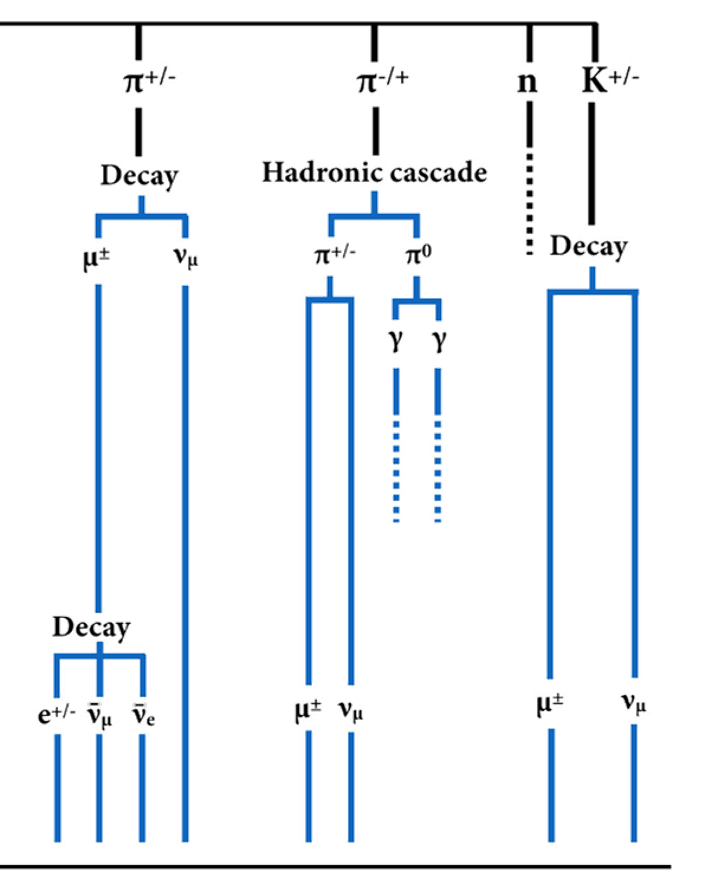
\includegraphics[width=9cm]{hadron_cascade.png}
		\caption{A portion of the cascade down from cosmic ray collisions to decays to leptonic particles. Taken from the Junior Lab CosmicWatch lab manual \cite{labmanual}.}
		\label{fig:cascade}
	\end{figure}

	Due to the non-abelian nature of the underlying $SO(3)$ group generators of quantum chromodynamics, the theoretical framework of the strong force, the upper-atmospheric collisions cause a hadronic cascade, i.e. a shower of particles which continually decay to new daughter particles. Figure~\ref{fig:cascade} displays a portion of one such cascade wherein dimuons pairs $\mu^{\pm}$ are seen as the resulting particles from three of the decays.
	
	Despite their very short lifetimes, muons are still observed on the surface of the Earth despite having to travel several kilometers from their points of origin in the upper atmosphere. Due to their relativistic speeds, their Lorentz factor $\gamma=\frac{1}{\sqrt{1-\frac{v^{2}}{c^{2}}}}$, they experience significant time dilation, which allows them to reach Earth's surface before they decay.

 	The Particle Data Group predicts that, at near ground level, the angular distribution of muons is of the form $I\propto\cos^{2}(\theta)$ \cite{pdg}. In figure~\ref{fig:model}, we display a theoretical model of the normalized average muon count rate as a function of elevation angle.
	\begin{figure}
		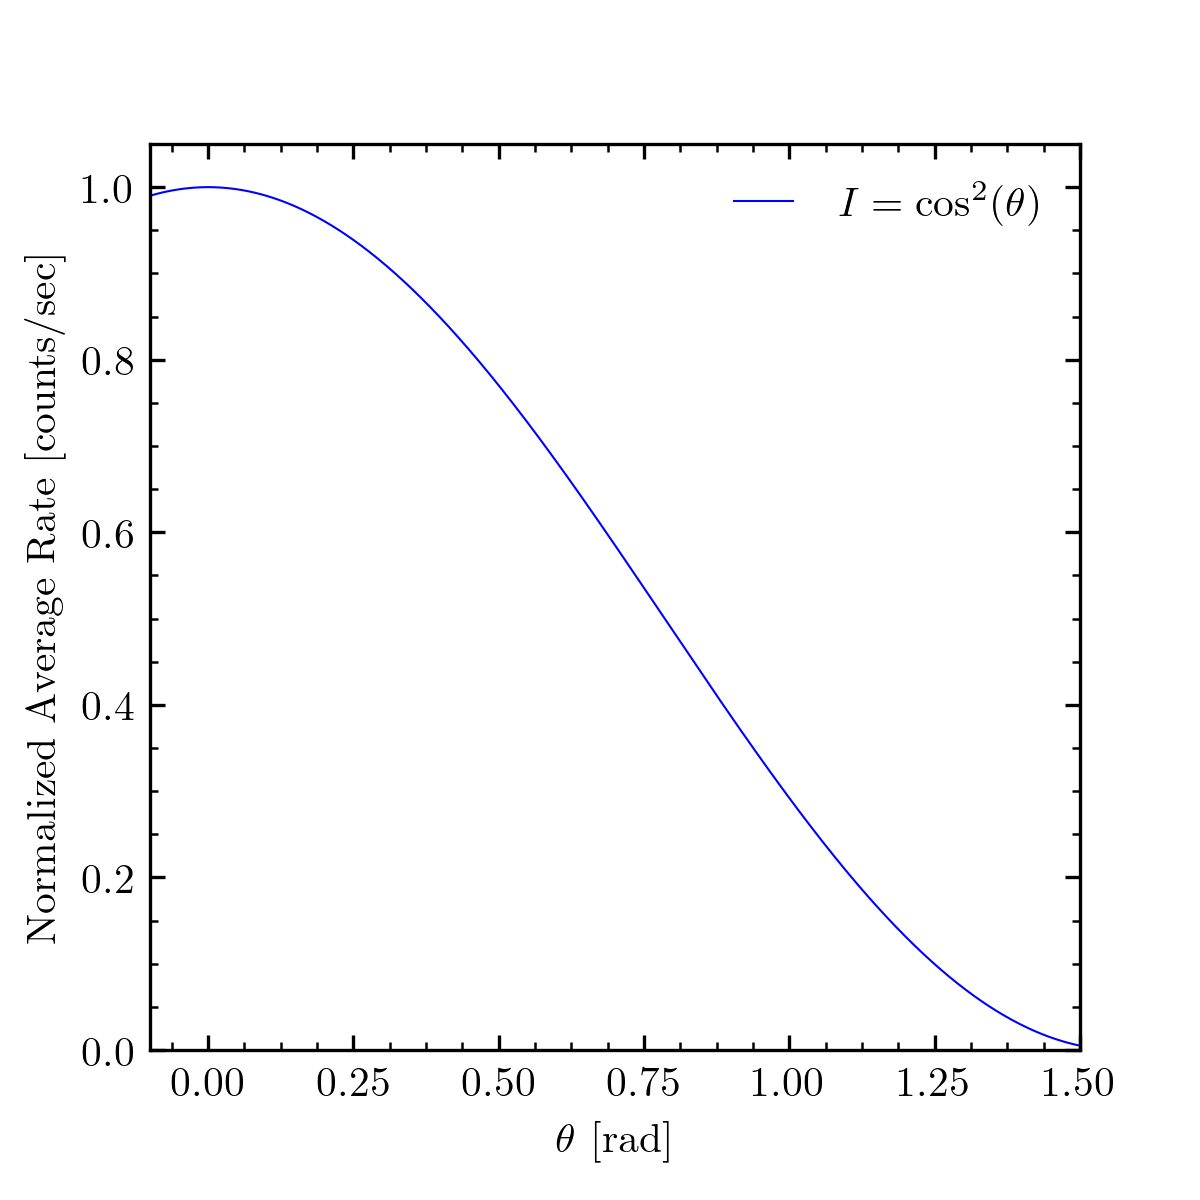
\includegraphics[width=9cm]{theor_avg_vs_theta.png}
		\caption{A theoretical plot of the functional form of average muon count rate as a function of angle.}
		\label{fig:model}
	\end{figure}
	We take the above function to be the model to which we will compare our data, and will use it as the functional form of best-fit to determine best-fit parameters $a$ and $b$ for $f(\theta)=a\cos^{2}(\theta)$.
	
	
	%%%%%%%%%%%%%%%%%%%%%%%%%%%%%%%%%%%%%%%%%%%%%%%%%%%%%%%%%%%%%%%%%%%%%%%%
	\section{Experimental Procedure}

	\subsection{The CosmicWatch Circuitry}
	Although the details of the CosmicWatch's inner circuitry are rather complex, there are a few salient details we can extract from the device's construction to understand the high-level function of the detectors.
	
	The first major piece of hardware in the CosmicWatch detectors is the scintillator. When muons arrive at the detector, they traverse through scintillator, i.e. a luminescent material upon exposure to ionizing radiation, emitting light. The other components of the circuitry are able to extract useful information from this scintillation light.
	
	The second crucial component of the CosmicWatch circuitry is the silicon photomultiplier (SiPM), which is a photon-sensitive device that detects the scintillation light and transmits this signal through the printed circuit board (PCB). Then, the microcontroller in the circuit measures the time and amplitude of the signal to confidently determine whether a muon has successfully been detected. 
	
	\begin{figure}[H]
		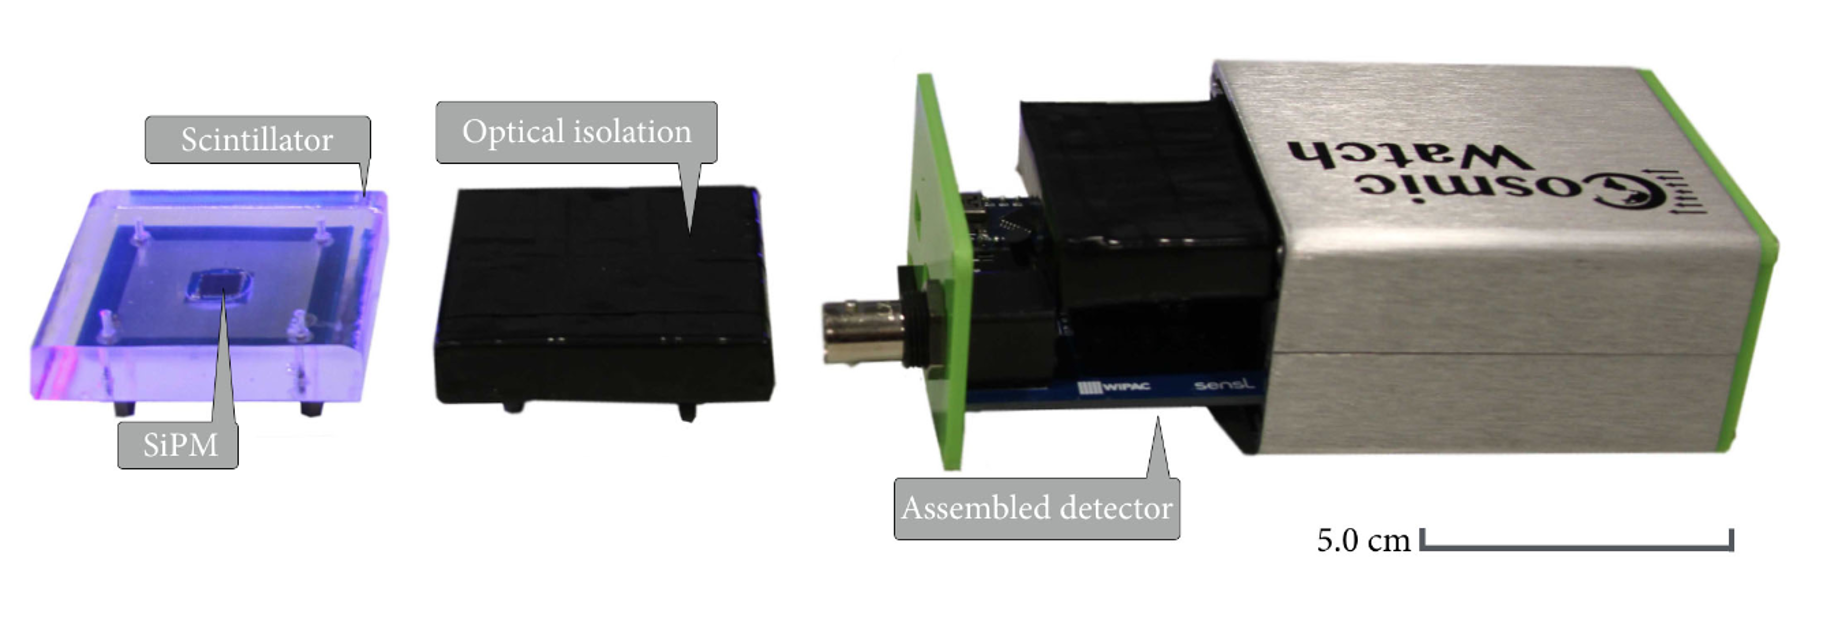
\includegraphics[width=8cm]{cosmicwatch_comps.png}
		\caption{Components of the CosmicWatch detector. The SiPM and the scintillator are seen on the left, which are internal to the detector whose full form is seen on the far right. Taken from \cite{labmanual}.}
		\label{fig:components}
	\end{figure}
	
	
	\subsection{The Apparatus}
	Our apparatus consists of two CosmicWatch detectors, a platform on which to secure them and tilt, and a protractor used to measure angles of elevation. We use a cardboard box as our platform, and use tape to secure the detectors to its surface. It should be noted that we choose to stack the two detectors on top of one another, as opposed to any other configuration. We will discuss the consequences of this choice further in our section on error analysis.
	
	We place the cardboard box on the surface of the laboratory table in the Junior Lab and use the adjacent wall as the surface against witch to tilt the box, so as to increase the elevation angle of the detectors. 
	
	\begin{figure}[H]
		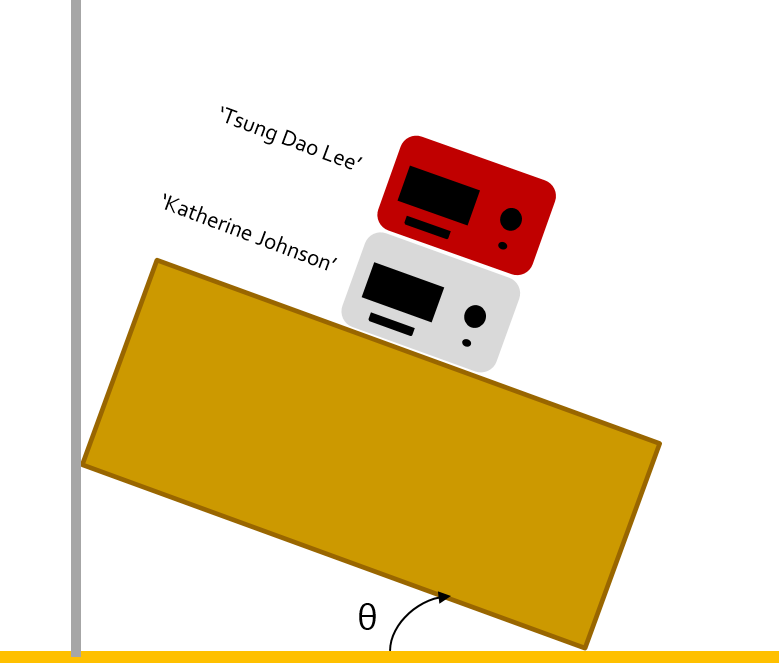
\includegraphics[width=8cm]{setup_diagram.png}
		\caption{A diagram of our physical lab setup}.
		\label{fig:setup}
	\end{figure}
	

	\subsection{Measurement Procedure}
	
	We perform measurements for seven different angles, ranging from $0^{\circ}$ to $60^{\circ}$ in increments of $10^{\circ}$. At each of the angles, we allow the detectors to collect data for 12 minutes with the detectors set to coincident mode. To measure the angles of elevation $\theta$, we use a laboratory protractor which makes measurements up to a precision $\pm 1^{\circ}$. We take this to be our uncertainty in angle measurements, i.e. the uncertainty in the dependent variable. 

	%%%%%%%%%%%%%%%%%%%%%%%%%%%%%%%%%%%%%%%%%%%%%%%%%%%%%%%%%%%%%%%
	\section{Data and Error Analysis}
	
	
	In this section I present raw data collected, as well as our reduced data followed by a discussion on the relevant errors and their sources. 
	
	\subsection{Accrued Muon Counts}
	
	We begin by examining the accumulated muon counts, i.e. the sum of all muon counts over time at each point in time. 
	 
. 	\begin{figure}[H]
		\centering
		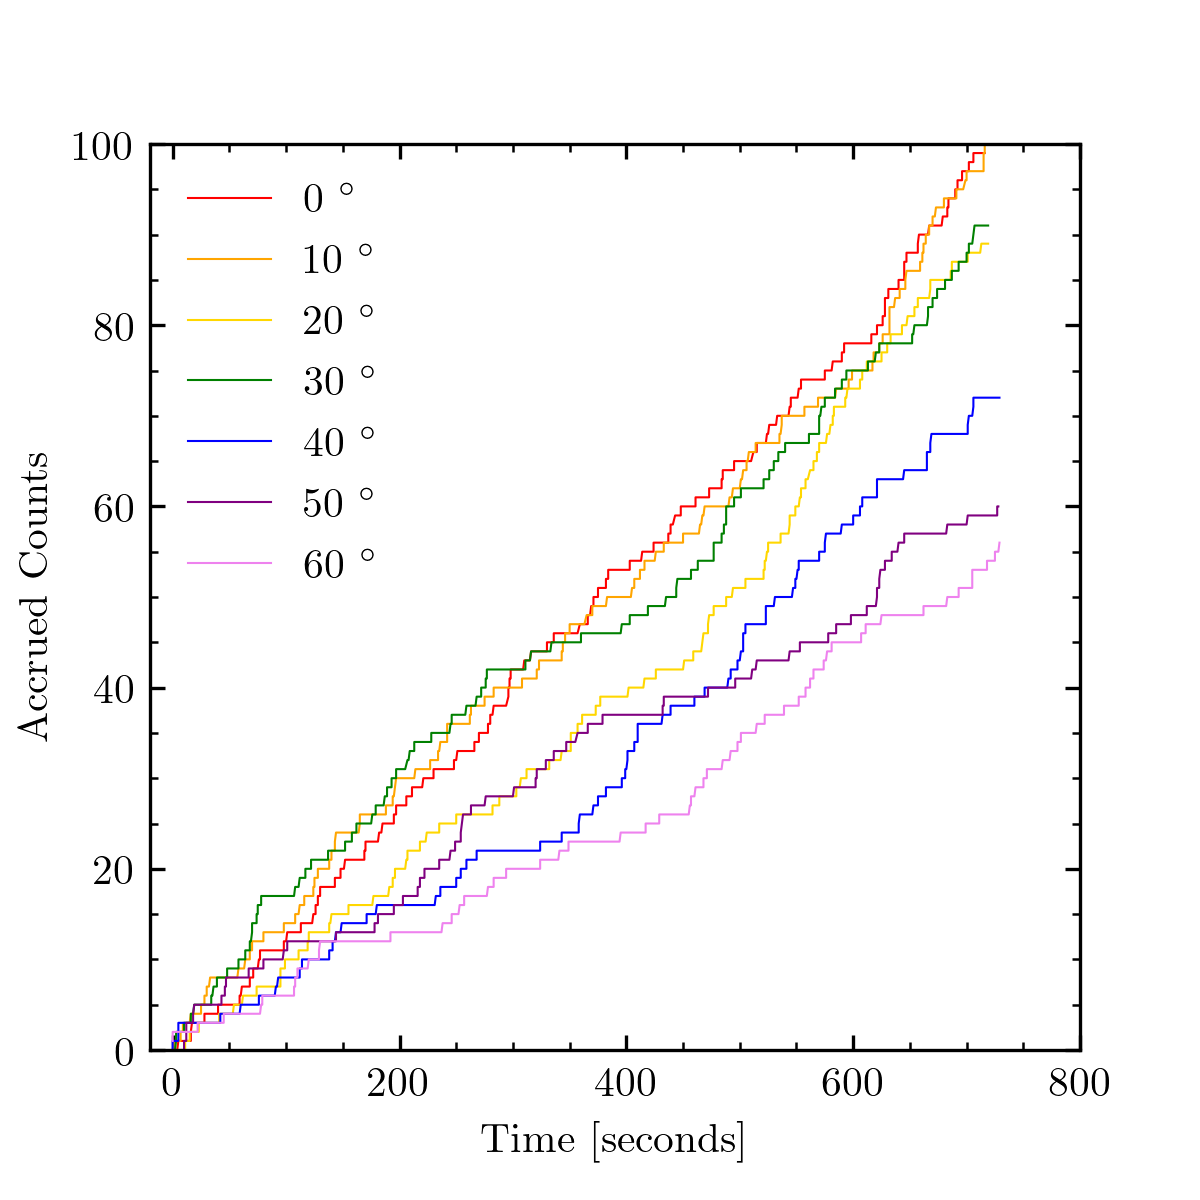
\includegraphics[width=9cm]{cum_sum_all.png}
		\caption{All seven cumulative muon counts for each of the elevation angles, color-coded according to the legend.}
		\label{fig:all_cumsum}
	\end{figure}
	In figure~\ref{fig:all_cumsum}, we see the cumulative muon counts for all seven angles. Though there is some fluctuation for each of the datasets across the 12 miuntes of data collecting, we observe the general trend that by the end of the period the lower angles demonstrate higher total muon counts, decreasing consistently with increasing angle of elevation. 
	
	After examining the accrued counts of detected muons over time, we consider the cumulative averages for each of the seven datasets. As we would already expect based on our results above, we predict that the cumulative averages for each of the angles will steady out over time such that the lower angle data will exhibit the highest average muon count rates, and decrease as the angles increase.
	
	\begin{figure}[H]
		\centering
		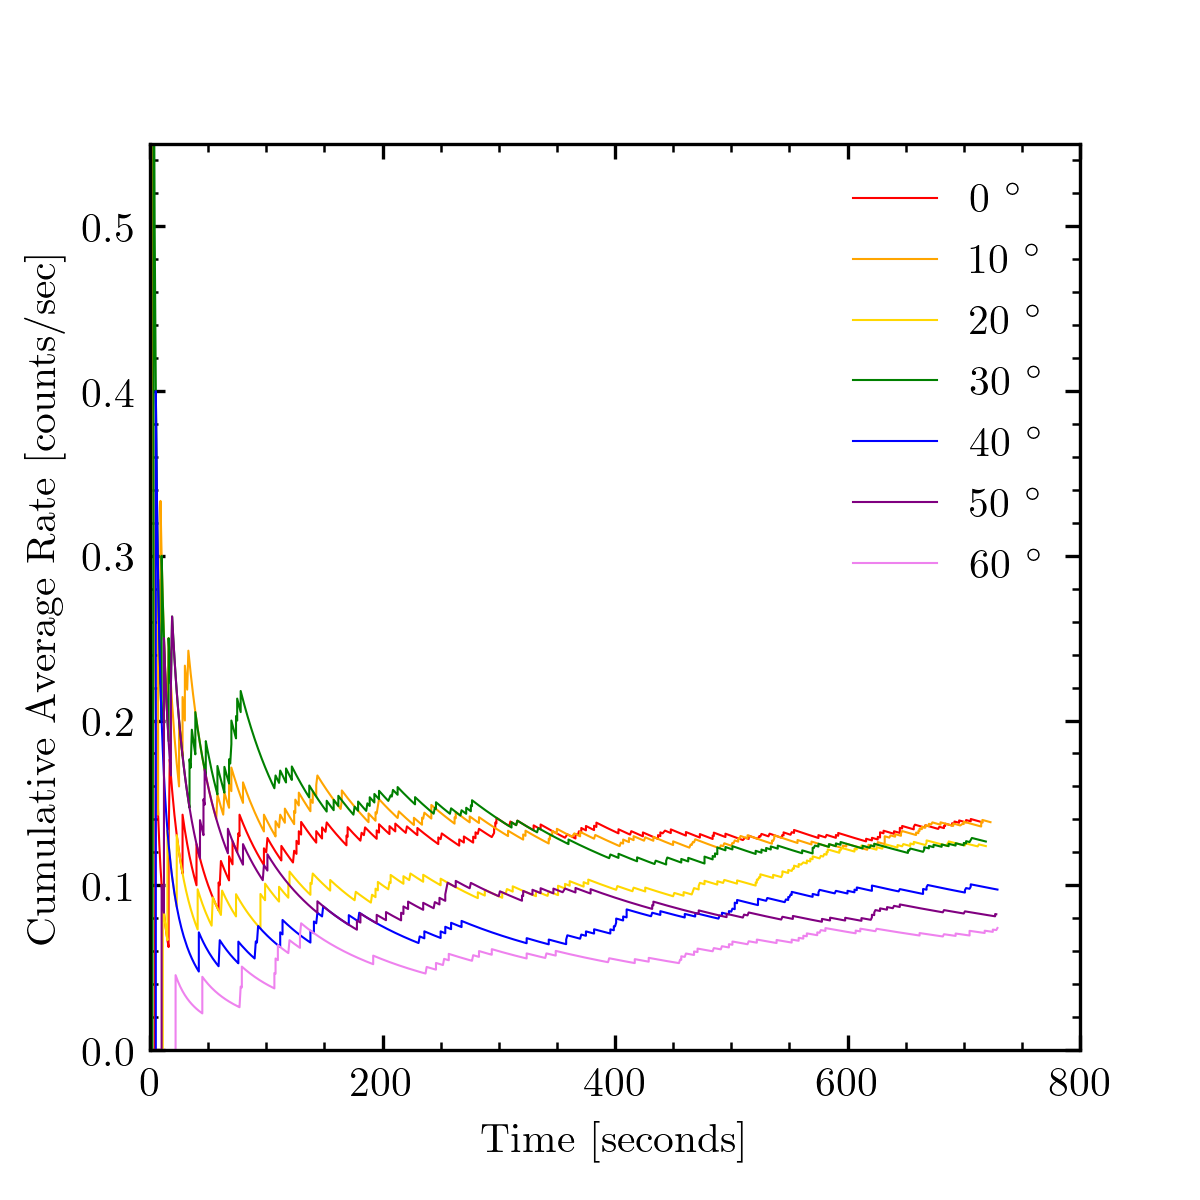
\includegraphics[width=9cm]{cum_avg_all.png}
		\caption{All seven cumulative average muon count rates over time.}
		\label{fig:all_cumavg}
	\end{figure}

	As seen in figure~\ref{fig:all_cumavg}, the cumulative average data at earlier times exhibits statistical fluctuations due to the shorter periods of time by which the muon counts are divided. Then as time continues, these fluctuations dampen and each of the seven cumulative averages approaches a steady number. We take the final data point of this curve, i.e. $\frac{\mathrm{Total muon counts}}{12 minutes}$, to be the overall average muon count rate for each angle. 	
	
	\subsection{Observed Angular Dependence of Count Rate}
	Having calculated the average muon count rates for each of the seven angles, we can construct a plot from these data to examine our experimental angle-dependent muon spectrum. 
	\begin{figure}[H]
		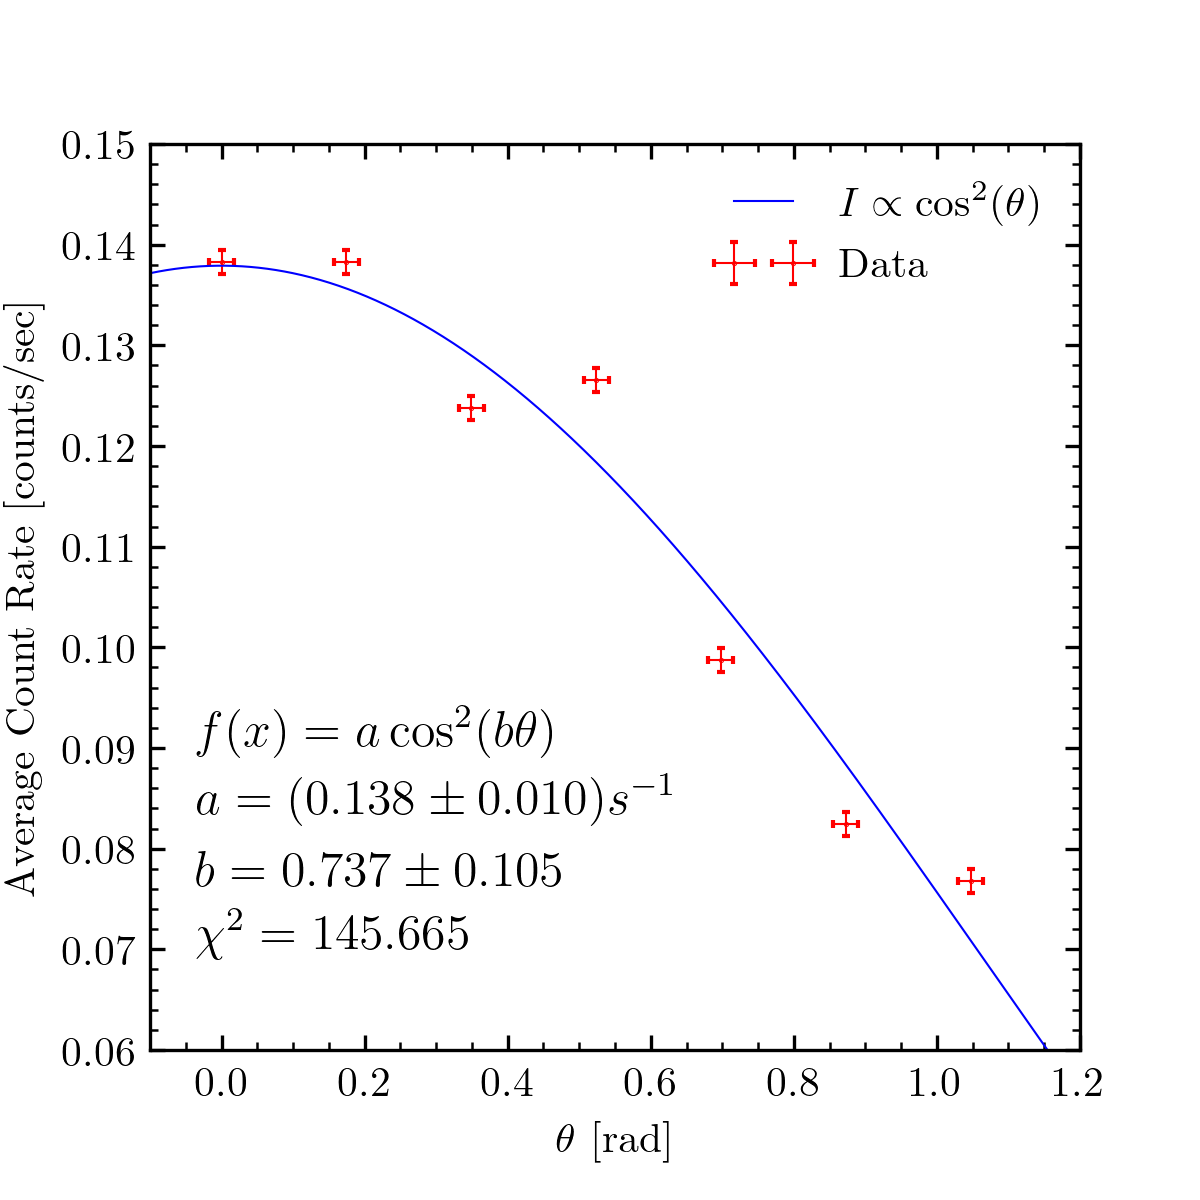
\includegraphics[width=9cm]{rate_vs_theta_fitted.png}
		\caption{The calculated average muon count rates at each elevation angle, with the best fit function and fit parameters displayed as well.}
		\label{fig:ang_fit}
	\end{figure}
	In figure~\ref{fig:ang_fit}, we show the data points for average muon count rate versus elevation angle $\theta$, where the angle is now in radians along the x-axis. We also display our function of best fit, taking the same form as discussed in section I.1. 
	
	Our best fit parameter $a=(0.138\pm0.010)s^{-1}$, which very closely approximates the average count rate at the elevation angle of 0. Hence, the sinusoidal amplitude of the unnormalized angular muon spectrum is determined by its count rate when the detectors are not at an angle.
	
	Moreover, our fit function with 5 degrees of freedom appears to be a good fit for the data, with a chi-squared value of $\chi^{2}=145.665$.
	
	
	\subsection{Error Estimation and Discussion}
	I attribute contributors to statistical uncertainties throughout this experiment mainly to the scarcity of data:
	\begin{itemize}
		\item we only perform one data collection period for each angle, and therefore only derive one average muon count rate. 
		\item we observed greater statistical fluctuations in the cumulative averages for each angle due to the brevity of each data collection period, each of which only lasted 12 minutes
		\item there is always a small chance, regardless of detector orientation, of erroneous muon counts coming from accidental coincidences recorded by the muon detectors. This becomes more of a systematic error when the muon detectors are separated at spaces that are too great for coincidence measurements to accurately occur.
	\end{itemize}
	
	I attribute the sources of the systematic uncertainty to a number of factors as well:
	\begin{itemize}
		\item We place our detectors on top of one another rather than side by side, meaning there is a larger subtended angle above them through which muons may arrive simultaneously, so coincident muons are not originating from a small region of the sky. Thus measuring the angular response is less meaningful with such a regime, as the angular dependence is sharper when muons originate from a smaller region of the sky
		\item the larger subtended angle from the detector configuration also leads  to more erroneously reported coincident muons, since the muon detection rates are artificially high 
	\end{itemize}  
	
	
	%%%%%%%%%%%%%%%%%%%%%%%%%%%%%%%%%%%%%%%%%%%%%%%%%%%%%%%%%%%%%%
	\section{Conclusions}
	In sum, we used the desktop muon detectors to successfully probe the dependence of the observed count rate on the angle of elevation at which the detectors are tilted. .
	
	These results provide an important accentuation to other studies of the dependence of muon count rates on elevation and on shielding materials. In addition, muons are crucial particles used to test modern particle physics for evidence of phenomena beyond the Standard Model \cite{muons}. Understanding the angular dependence of muon count rates is an important step in designing powerful particle detectors at energy scales comporable to the Large Hadron collider (LHC) such that cosmic ray muon backgrounds can be separated from the muons resulting from proton-proton collisions, for example.
	
	Much more can be studied with these tools and results. With more trials for each angle and greater data collection time, we can replicate these results with greater fidelity to the same predicted model or show instead that perhaps the dependence follows another functional form
	
	%%%%%%%%%%%%%%%%%%%%%%%%%%%%%%%%%%%%%%%%%%%%%%%%%%%%%%%%%%%%%%%%%%%%%%%
	\begin{acknowledgments} The author is very grateful to Luke Gianni for serving as his lab partner throughout this experiment. The author is also very thankful for the constructive feedback offered by Professor Fakhri. The author would additionally like to thank Hanzhen Lin for their useful discussions on various related topics. 
	\end{acknowledgments}
	
	%%%%%%%%%%%%%%%%%%%%%%%%%%%%%%%%%%%%%%%%%%%%%%%%%%%%%%%%%%%%%%%%%%%%%%%%% 
	
	\bibliography{paper3}
	
\end{document}
